The system allows farmers to access the personalized best practice data base on their location and type of production. To analyze farmers' performances, they are required to fill the result sometimes.(Better to specify everyday, every week..?) There are the pages where they could exchange their opinion among famers, ask suggestion for agronomists by sending messages. 
\newline
On the other hand, the system serves agronomists to let them answer the request from farmers. 
Agronomists need to register their responsible area, according to the registered area the system organize the visits plan and notify them. The provided plans are able to be modified if there is the needs from agronomist, and it will be also tracked the meeting statuses.(Understandable?)
\newline
Lastly for policy maker, the system provides only visualization function. The available data are the
classification of farmer according to their performance, places with critical natural disaster, statuses of the incentives for awarded farmers, and outcome of agronomist visits for low performance farmers. Considering their jobs, since farmers need to be outside most of the time, using smartphone application would be suitable for them by the aspect of portability. Instead agronomists and policy makers, they mainly work inside therefore the desktop based web application will be provided. 
\newline
\newline
Here we would like to introduce a few pages to show how the application look like on main functions. The first and second one show sign up and sing in pages, which are common for all type of users. The third and forth ones serve for farmers to let them insert the production result. Lastly fifth one visualize the chat page between a farmer and an agronomist. We will present more in detail again in our Design Document. 

\begin{figure}[H]
	\centering
    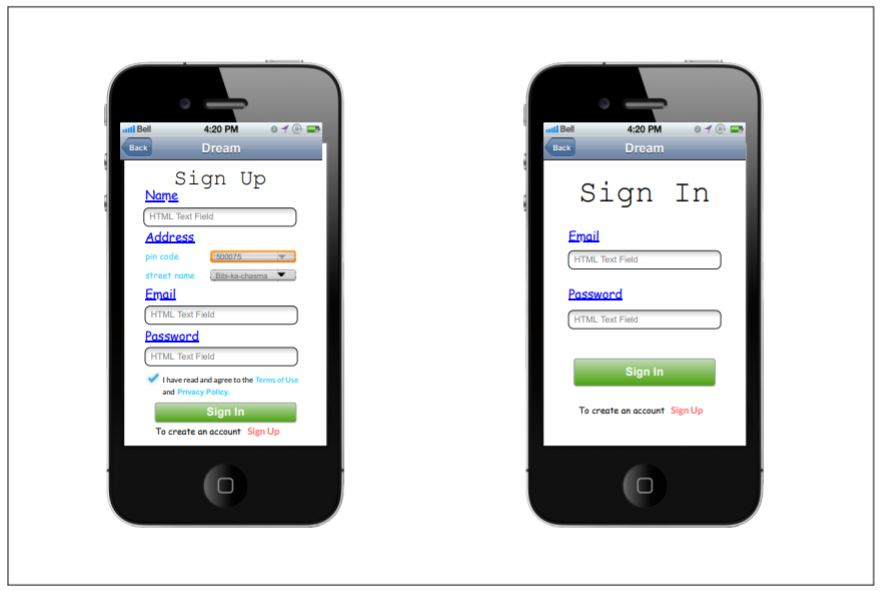
\includegraphics[page=1, width=\textwidth]{Images/sign_up_in.JPG}
	\caption{\label{fig:FE_image}Sign Up, Sign In}
\end{figure}

\begin{figure}[H]
	\centering
    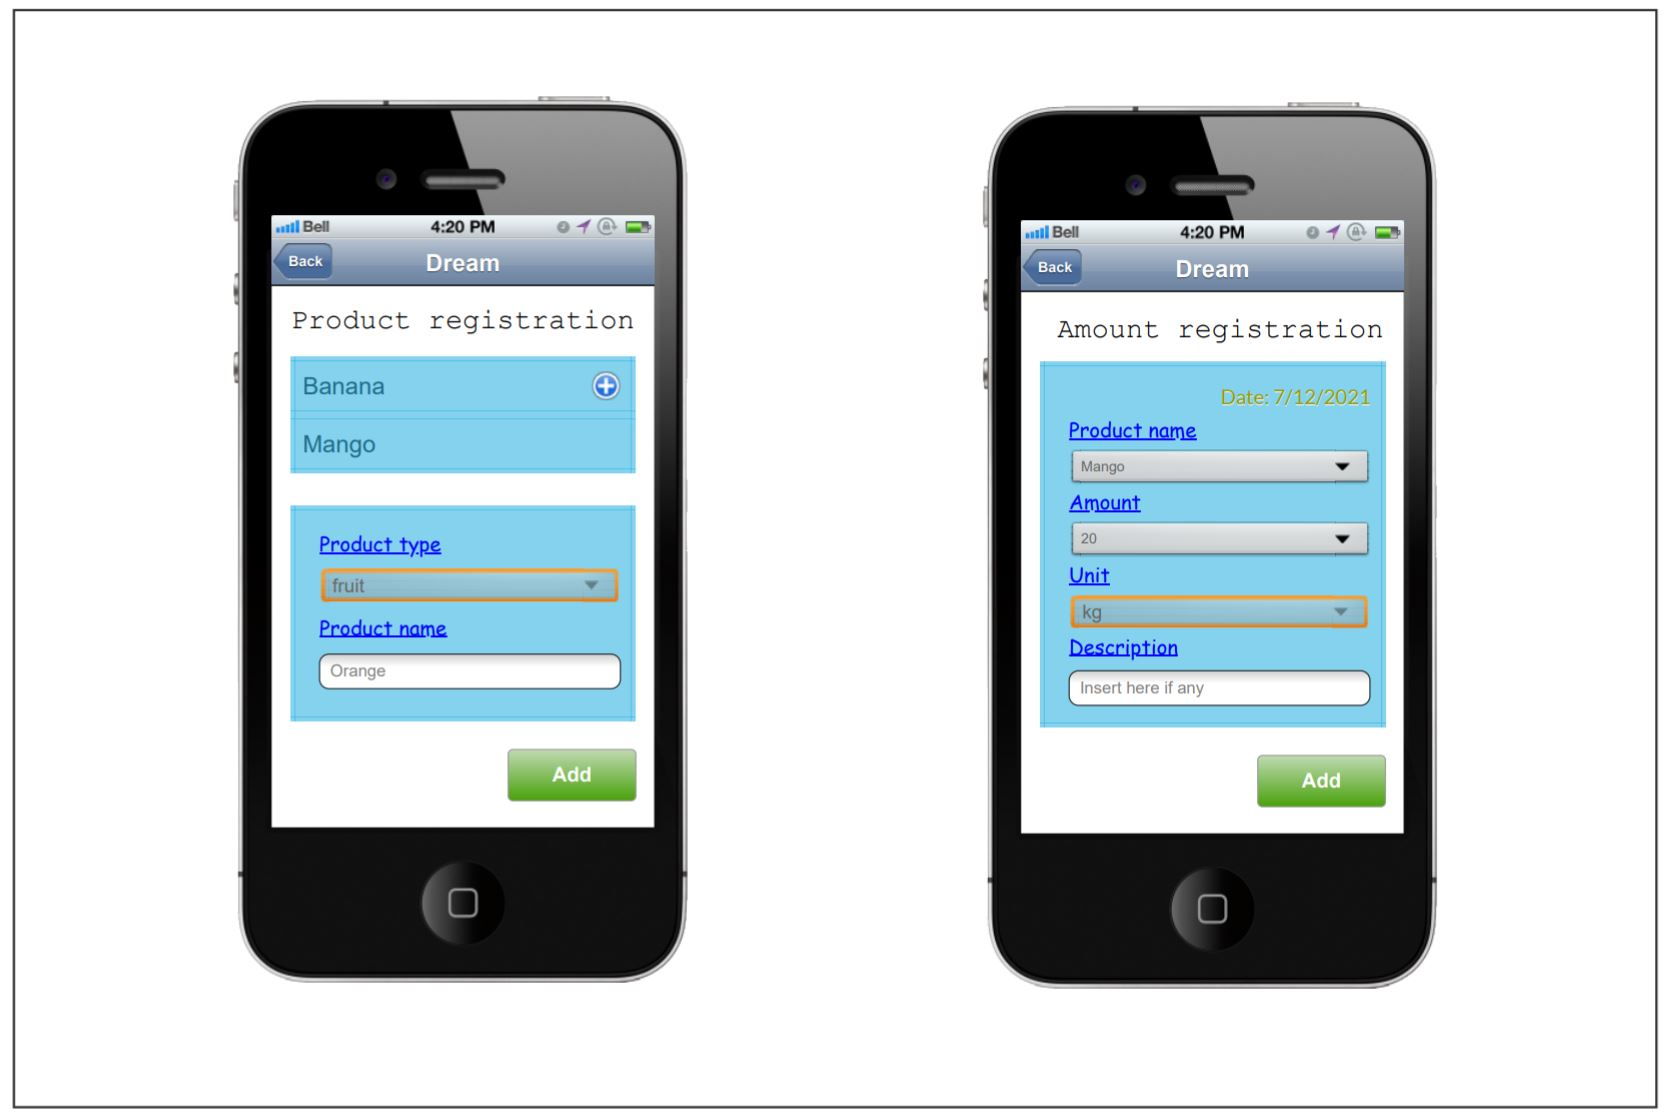
\includegraphics[page=1, width=\textwidth]{Images/product_amount_registration.JPG}
	\caption{\label{fig:FE_image}Product registration, Amount registration}
\end{figure}



\begin{figure}[H]
	\centering
    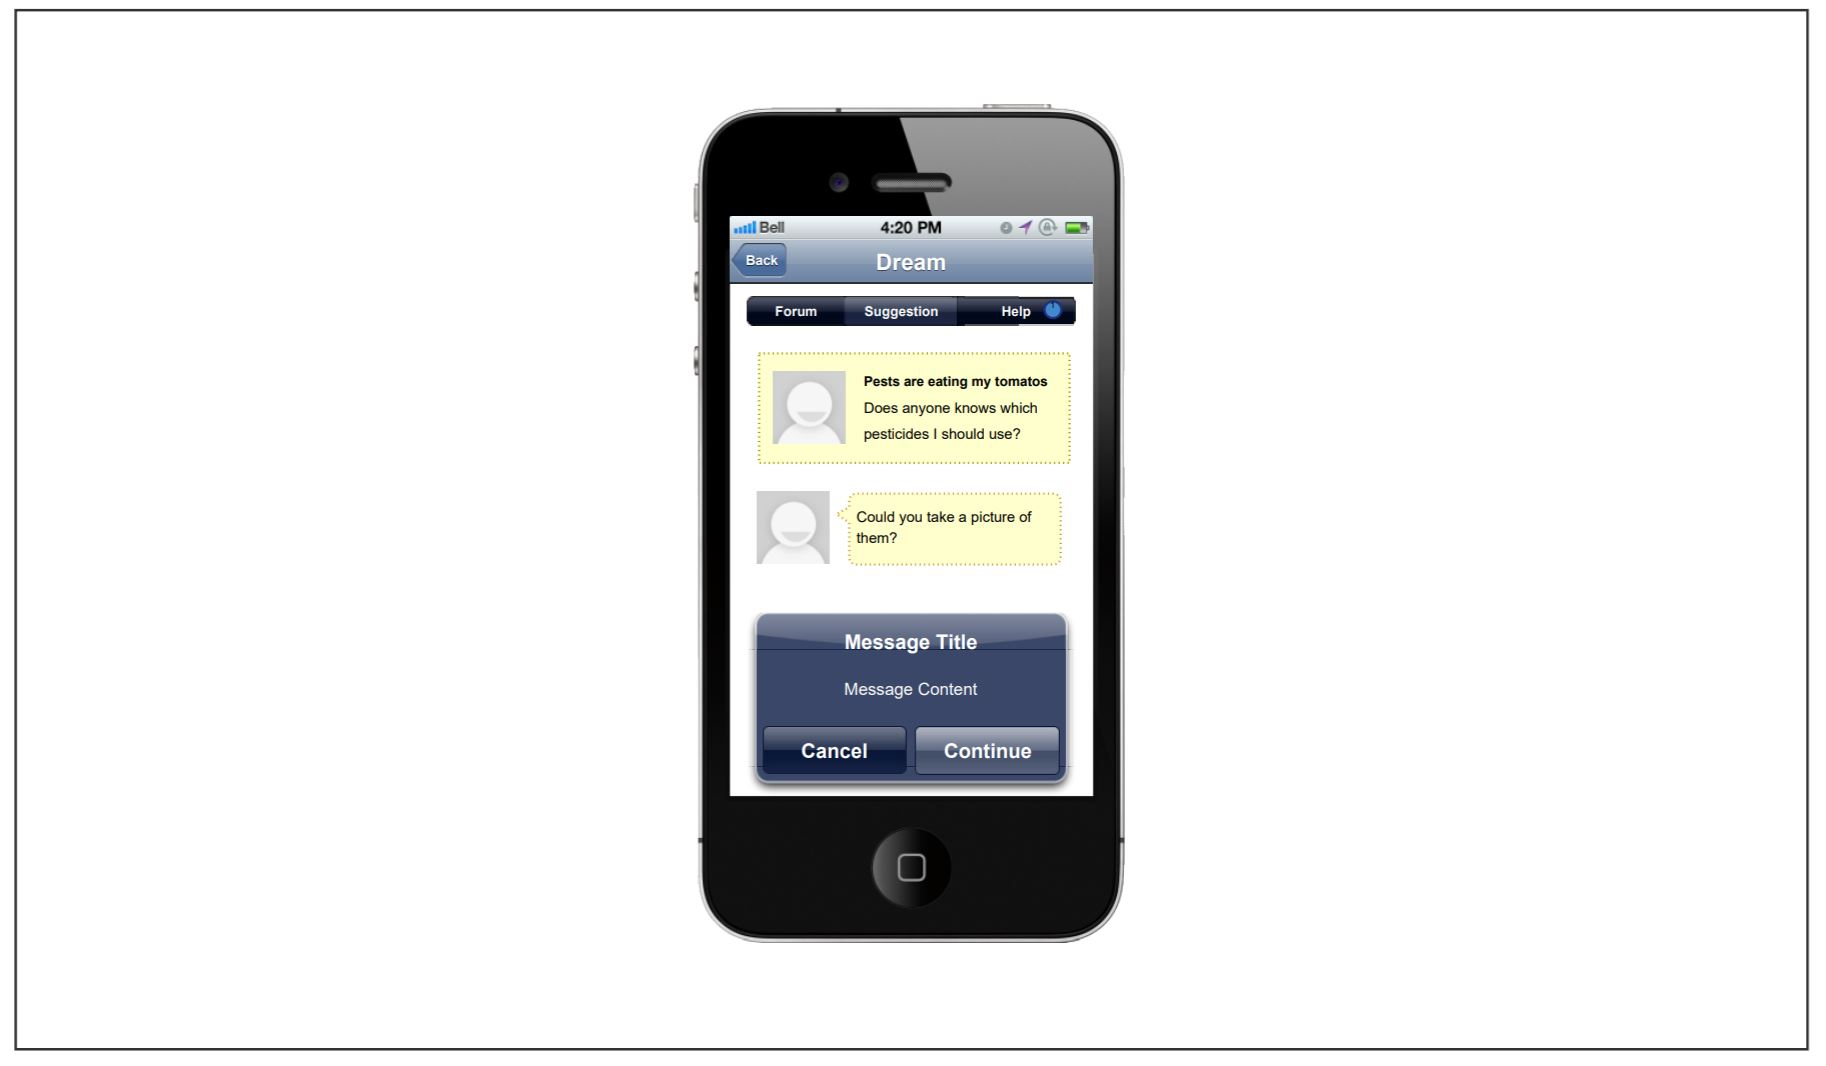
\includegraphics[page=1, width=\textwidth]{Images/message_insertion.JPG}
	\caption{\label{fig:FE_image}Message insertion}
\end{figure}

\begin{figure}[H]
	\centering
    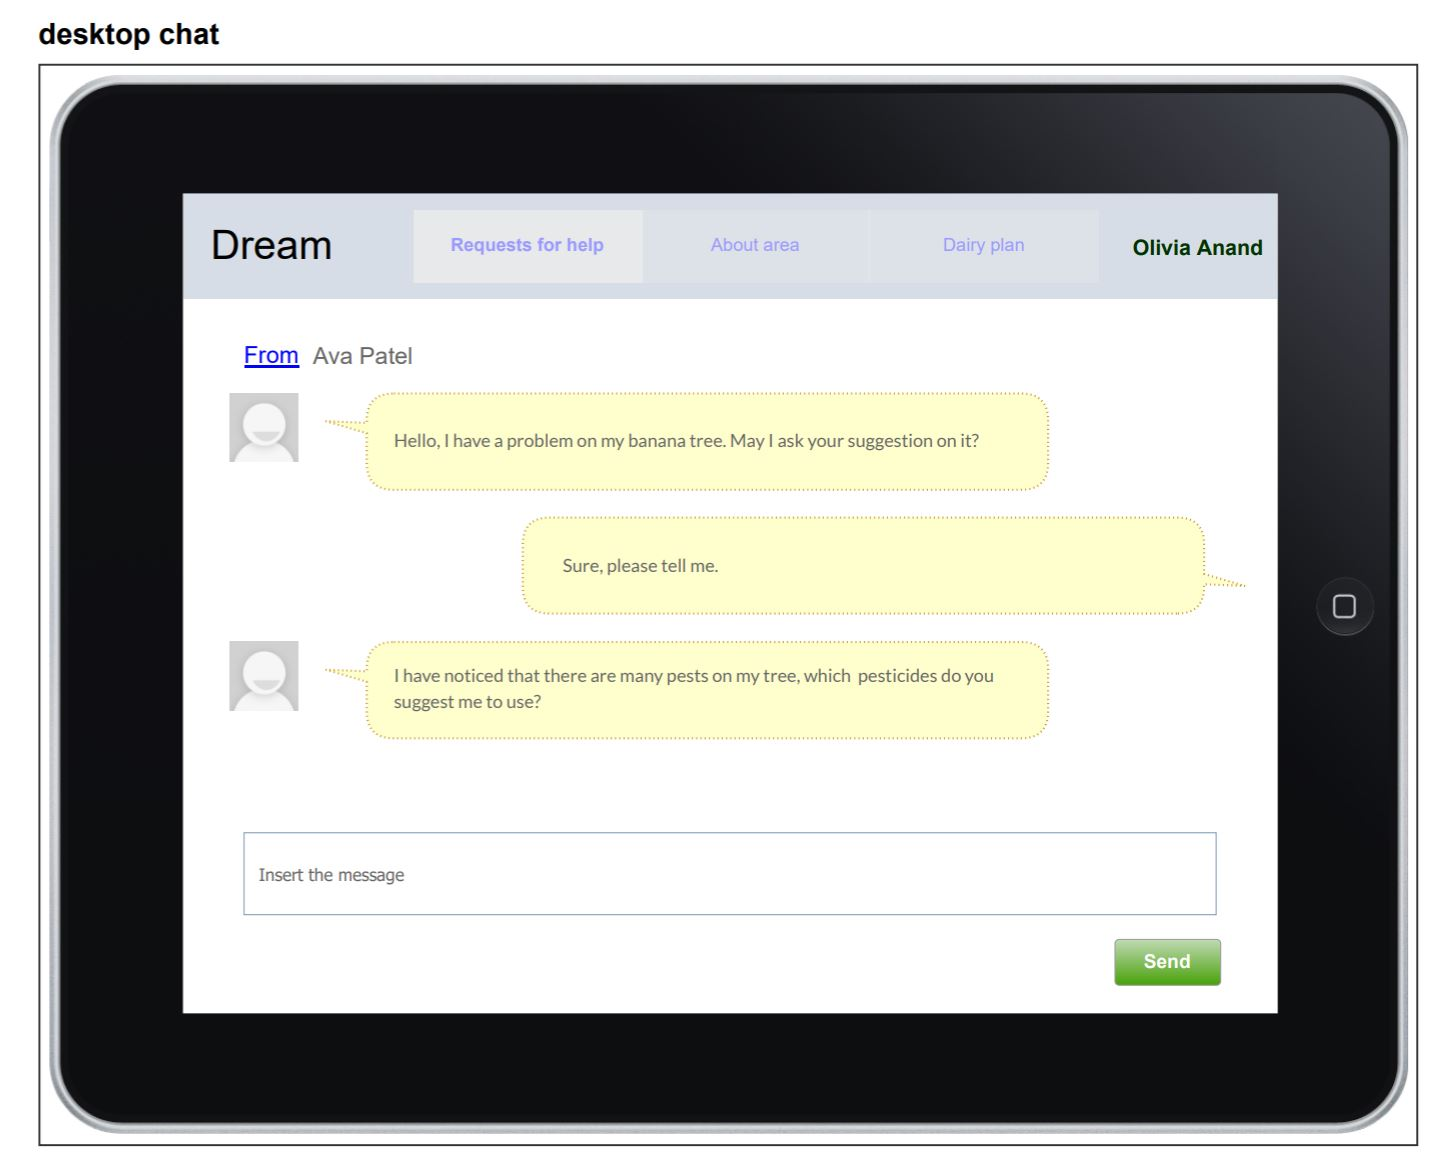
\includegraphics[page=1, width=\textwidth]{Images/desktop_chat.JPG}
	\caption{\label{fig:FE_image}Desktop chat}
\end{figure}